\section{MIMO in handsets} % (fold)
\label{sec:mimo_in_handsets}
Multiple-input and multiple-output (MIMO) is a convenient way to deal with the challenges in delivering more throughput and coupe with the multipath effectcs from buildings etc. The purpose of this section is to explain what is understood by such a system, how it relates to the antenna design and how it makes a difference. The principal mechanisms and performance metrics are explained. This section will not desribe the statistical channel models, but rather focus on the antenna related perspectives. 

\begin{figure}[htbp]
  \centering
  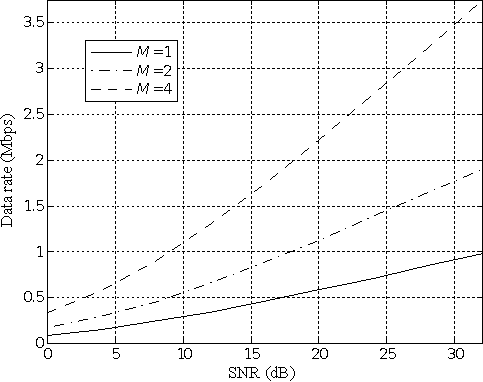
\includegraphics[width=\textwidth]{img/datarateMimo}
  \caption{Throughput versus SNR given a specific M-ary MIMO-setup\cite{Ezio2007MIMO}}
  \label{fig:mimo-throughput}
\end{figure}

\subsection{Perks of MIMO} 
As shown in the introduction to this section, the use of MIMO comes with enhancement in performance. Figure~\ref{fig:mimo-throughput} showed the general performance increase, however this is gained by the addition of multiply different performance gains. These are spatial diversity gain, multiplexing gain, arrary gain and interferende reduction\cite{Ezio2007MIMO}, which will be described breifly in the following.


\subsubsection{Spatial Diversity Gain}
The spatial diversity gain, improves the resistance to fading in the receiver. This is done by providing the receiver with multiply different copies of the same transmitted signal, ideally the copies are independent from another. A diversity tecnique is required to combine the signals at the receiver\cite{Ezio2007MIMO}, some examples could be equal gain combining, maximal-ratio combining or selection combining. This diversity is also quite intuitive since the probability that one of the signals are not in a fade increases per added element, given that they are somewhat independend. 
 
\subsubsection{Spatial Multiplexing Gain}
Spatial multiplexing can be used in scatter rich channels, where each received signal are independend. Instead of transmitting the same signal, as with the diversity gain, the spatial multiplexing transmits multiple independent data stream, thus this allows for a linear increase in the data rate thus the capacity of the wireless network is increased. Generally the number of independent streams that can be supported are limited by the number of receive antennas. 

\subsubsection{Array Gain}
The array gain is the result of coherent combining of the wireless signals at the receiver, which results in an increase in the receive SNR. The arrary gain is improved by the number of antenna elements until a certain saturation point. This gain improves the resistance to noise and thus also the coverage. 
  
\subsubsection{Interference Gain}
By using MIMO the interference from different users and basestations can be avoided by exploting extra spatial degrees of freedom, such as arrary gain. Furthermore one could imagine that beamsteering could be implemented such that the signal could be directed towards the designated receiver. Obviously all of the above can not be used at the same time, however using a combination of this allows for improved coverage, capacity or reliability.
 
\subsection{Antenna Design in MIMO Applications}
The three most important factors in MIMO antenna design are: near-field coupling, the envolope correlation $\rho_e$ and total efficiency $\eta_{total}$. The near-field coupling which is a measure of the coupled power towards the second antenna when the first antenna is excited, which is evaluted by the $S_{21}$ parameter, this is also often refered to as the isolation. This isolation affects the efficiency and envolope correlation coefficient~\cite{Tatomirescu2011PortIsolation}. 

The total efficiency is simply given by Equation~\ref{eq:mimo_total_eff}\cite{Tatomirescu2011PortIsolation}, where $\eta_{rad}$ is the radiation efficiency, which takes dielectric and conductive lossed into acocunt. 

The envelope correlation coefficient can be calculated by Equation~\ref{eq:envlop_corr} \cite{Tatomirescu2011PortIsolation}. The far-field radiation pattern needs to be measured in order to reliably calculated the envelope correlation coefficient.

\begin{align} 
\rho = \frac{\oint(\text{XPD} \cdot E_{\theta X}(\Omega) \cdot) E^*_{\theta X} \cdot p_\theta(\Omega)+E_{\phi Y}(\Omega) \cdot) E^*_{\phi Y} \cdot p_\phi(\Omega) )d\Omega}{\sqrt{\oint(\text{XPD}\cdot G_{\theta X}(\Omega) \cdot p_\theta(\Omega)+G_{\phi X}(\Omega) \cdot p_\phi(\Omega))d\Omega \cdot \oint(\text{XPD}\cdot G_{\theta Y}(\Omega) \cdot p_\theta(\Omega)+G_{\phi Y}(\Omega) \cdot p_\phi(\Omega))d\Omega }}
\end{align}

Equation~\ref{eq:envlop_corr} assumes uniform 3D angular power spectrum of the received signal and is not valid if this is not the case. The envelope correlation coefficient can also be estimated by the S-parameters, as given in Equation~\ref{eq:envlop_corr_Sparams}\cite{Alain2010MIMO}. However the use of this is often discouraged since it assumes very high radiation efficiency. 

\begin{align}
  \rho_e \approx |\rho_c|^2 = \frac{|S^*_{11}S_{12}+S^*_{21}S_{22}|^2}{(1-|S_{11}|^2-|S_{21}|^2)(1-|S_{22}|^2-|S_{12}|^2)}
\end{align}

Thus, when designing antenna for the purpose of MIMO, they need to be designed in a way such that the elements receives de-correlated signals, this can be in different ways, such as changing the angular patterns or polarization of the elements or spatially seperating the antennas, these are the most used however there are also other tecniques such as decoupling networks, parasitic elements, active antenna cancelation, eigen modes and balanced currents. 

\subsubsection{Spatial Correlation}
The spatial correlation between two antennas  is given by the radiated E-field patterns as given in Equation~\ref{eq:envlop_corr}. There it is seen that the correlation is a comparison between the radiated E-field patterns and the incident E-fields arriving at the antenna, which is given by the probability $p_\thega$ and $p_\phi$. 

From the Equation~\ref{eq:envlop_corr} it can also be deduced that the spacing, polarisation and radiation patterns all effect the correlation between two antennas. In order to investigate the only effects of spacial seperation we consider the case with two omnidirectional antennas both purely vertically polarized. This can be described by Equation~\ref{eqn:spactial_corr}\cite{Tim2012Practical}, where $d$ is the horizontal spacing and $l$ is the vertical spacing. 

\begin{align}
  \rho = \oint e^{j\beta \sqrt{d^2+l^2}\cos\zeta}p_\theta(\theta,\phi)\sin\theta \, \mathrm{d} \theta \mathrm{d} \phi
\end{align}

where: 

\begin{align}
\cos \zeta = \sin(\phi + \tan^-1(\frac{l}{d}) \text{sgn}\phi)\sin\phi  
\end{align}

In Figure~\ref{fig:spatial_correlation} two cases of Equation~\ref{eqn:spactial_corr} are shown, one where only the horizontal spacing is considered and another whre only the vertical spacing is considered. The angle of arrival is given by Taga, where the mean angle $\overline{\theta}$ is at \SI{70}{\degree} and the standard deviation $\sigma_\theta$ is \SI{20}{\degree}. From the plot it can be seen that the vertical spacing required for a certain correlation is larger than that of the horizontal spacing, this comes from the taga-model used for the angle of arrival, since its distribution is nonuniform. This can however not be used to argue that the antennas should be spaced horizontally, since smartphones often is operated both horizontally and vertically! 

It is also possible to make the array in other toplogies such as planar, circular or random, this is however not very practical for mobile devices given the current usage of low frequencies in telecommunication \SIrange{500}{2700}{MHz} as described in Section~\ref{Lasse LTE}.

\begin{figure}[htbp]
  \centering
  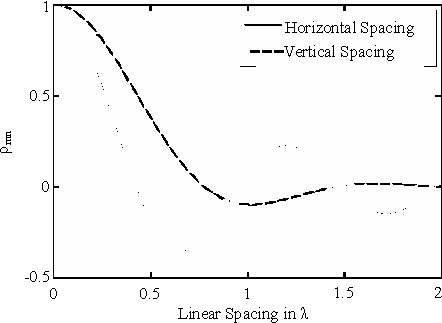
\includegraphics[width=\textwidth]{img/mimoSpacing}
  \caption{Spacing versus wavelength for the horizontal and vertical case\cite{Tim2012Practical}}
  \label{fig:mimo-spacing}
\end{figure}

\subsubsection{Other methods} %Nyt navn tak :D
In addition to the spatial seperation to decorrelate antennas, polarization and different radiation patterns can also be used to decorrelate elements. This is very often used in small mobile devices, where the physical size limits the spacing between elements.  

In theory using a perfectly polarized dipole and loop antenna, it would be possible to create total decorrelated elements, because they have opposite polarization. This is obviosuly hard to implement in practice, but it is possible to lower the correlation of to elements by having a difference in polarization. However using different polarizations to get a lower correlation requires a suitable XPR in the channel. The XPR should be around \SI{6}{dB} or lower\cite{Tim2012Practical}. 






 



% section section_name (end)

% chapter mimo_in_handsets (end)
%20458872 Jan SS